    \textbf{Задание №6} Выполнить индивидуальное задание для закрепления знаний на практике, подготовив соответствующую программу на языке С (номер задания соответствует номеру студента по журналу; если этот номер больше, чем максимальное число заданий, тогда вариант задания вычисляется по формуле: номер по журналу \% максимальный номер задания, где \% — остаток от деления; если остаток равен 0, студенту назначается задание с максимальным номером). \label{sec:6}

    \begin{minted}[frame=lines, framesep=2mm, baselinestretch=1.2, fontsize=\small, linenos]{c}
#define _GNU_SOURCE
#include <stdio.h>
#include <stdlib.h>
#include <string.h>
#include <errno.h>
#include <time.h>
#include <unistd.h>
#include <signal.h>
#include <sys/wait.h>
#include <sys/mman.h>

#define N          3
#define OPEN_SEC   2
#define CLOSE_SEC  3

static volatile sig_atomic_t *sent1, *sent2;
static volatile sig_atomic_t recv1 = 0, recv2 = 0, stop = 0;
static pid_t kid[N];
static sigset_t blk, old, empty;

static void h_usr1(int s)  { (void)s; recv1++; }
static void h_usr2(int s)  { (void)s; recv2++; }
static void h_int(int s)   { (void)s; stop = 1; }
static void h_alarm(int s) { (void)s; }
static void h_term(int s)  { (void)s; _exit(0); }

static void install(int signo, void (*h)(int), int flags)
{
    struct sigaction sa;
    memset(&sa, 0, sizeof(sa));
    sa.sa_handler = h;
    sigemptyset(&sa.sa_mask);
    sa.sa_flags = flags;
    sigaction(signo, &sa, NULL);
}

static void setup_shared_memory(void)
{
    size_t sz = N * sizeof(sig_atomic_t);

    sent1 = mmap(NULL, sz, PROT_READ | PROT_WRITE,
                 MAP_SHARED | MAP_ANONYMOUS, -1, 0);
    sent2 = mmap(NULL, sz, PROT_READ | PROT_WRITE,
                 MAP_SHARED | MAP_ANONYMOUS, -1, 0);

    memset((void *)sent1, 0, sz);
    memset((void *)sent2, 0, sz);
}

static void cleanup_shared_memory(void)
{
    size_t sz = N * sizeof(sig_atomic_t);
    munmap((void *)sent1, sz);
    munmap((void *)sent2, sz);
}

static void setup_parent_handlers(void)
{
    install(SIGUSR1, h_usr1,  SA_RESTART);
    install(SIGUSR2, h_usr2,  SA_RESTART);
    install(SIGINT,  h_int,   SA_RESTART);
    install(SIGALRM, h_alarm, 0);
}

static void setup_child_handlers(void)
{
    install(SIGINT,  SIG_IGN, 0);
    install(SIGUSR1, SIG_IGN, 0);
    install(SIGUSR2, SIG_IGN, 0);
    install(SIGTERM, h_term,  0);
}

static void setup_signal_masks(void)
{
    sigemptyset(&blk);
    sigaddset(&blk, SIGUSR1);
    sigaddset(&blk, SIGUSR2);
    sigemptyset(&empty);
}

static void child_loop(int id)
{
    srand((unsigned)(getpid() ^ (id * 2654435761u)));
    for (;;) {
        usleep((useconds_t)((100 + rand() % 301) * 1000));
        if (rand() & 1) {
            sent1[id]++;
            kill(getppid(), SIGUSR1);
        } else {
            sent2[id]++;
            kill(getppid(), SIGUSR2);
        }
    }
}

static void child_main(int id)
{
    setup_child_handlers();
    child_loop(id);
}

static void spawn_children(void)
{
    for (int i = 0; i < N; i++) {
        kid[i] = fork();
        if (kid[i] == 0)
            child_main(i);
    }
}

static void sum_sent(int *s1, int *s2)
{
    *s1 = 0; *s2 = 0;
    for (int i = 0; i < N; i++) { *s1 += sent1[i]; *s2 += sent2[i]; }
}

static void print_snapshot(const char *label)
{
    int s1, s2;
    sum_sent(&s1, &s2);
    printf("%s recv=(%d,%d) sent=(%d,%d)\n",
           label, recv1, recv2, s1, s2);
}

static void phase_open(void)
{
    print_snapshot("[OPEN]   начало:");

    time_t t0 = time(NULL);
    while (!stop && time(NULL) - t0 < OPEN_SEC) {
        alarm(1);
        sigsuspend(&empty);
    }
    alarm(0);

    print_snapshot("[OPEN]   конец: ");
}

static void phase_closed(void)
{
    sigprocmask(SIG_BLOCK, &blk, &old);

    printf("[CLOSED] сигналы заблокированы на %d с...\n", CLOSE_SEC);

    struct timespec ts = { CLOSE_SEC, 0 };
    while (nanosleep(&ts, &ts) == -1 && errno == EINTR)
        ;

    sigset_t pend;
    sigpending(&pend);

    printf("[CLOSED] pending: USR1=%d USR2=%d\n",
           sigismember(&pend, SIGUSR1) != 0,
           sigismember(&pend, SIGUSR2) != 0);

    int b1 = recv1, b2 = recv2;
    sigprocmask(SIG_SETMASK, &old, NULL);

    struct timespec pause = { 0, 200 * 1000 * 1000 };
    nanosleep(&pause, NULL);

    printf("[UNBLK]  из pending доставлено: USR1=%d USR2=%d\n",
           recv1 - b1, recv2 - b2);
}

static void run_cycle(int n)
{
    printf("\nЦикл %d\n", n);
    phase_open();
    phase_closed();
}

static void shutdown_children(void)
{
    install(SIGINT, SIG_IGN, 0);

    for (int i = 0; i < N; i++)
        kill(kid[i], SIGTERM);

    for (int i = 0; i < N; i++)
        while (waitpid(kid[i], NULL, 0) == -1 && errno == EINTR)
            ;
}

static void print_final_report(void)
{
    int s1, s2;
    sum_sent(&s1, &s2);
    printf("\nИтог: sent=(%d,%d) recv=(%d,%d) потеряно=(%d,%d)\n",
           s1, s2, recv1, recv2, s1 - recv1, s2 - recv2);
    printf("Обычные сигналы не встают в очередь: пока бит pending\n");
    printf("установлен, повторные такие же сигналы сливаются с ним.\n");
}

int main(void)
{
    setvbuf(stdout, NULL, _IONBF, 0);

    setup_shared_memory();
    setup_parent_handlers();
    setup_signal_masks();
    spawn_children();

    printf("Диспетчер %d, детей: %d\n", (int)getpid(), N);

    int cycle = 1;
    while (!stop)
        run_cycle(cycle++);

    shutdown_children();
    print_final_report();
    cleanup_shared_memory();
    return 0;
}
    \end{minted}

    \begin{figure}[H]
        \centering
        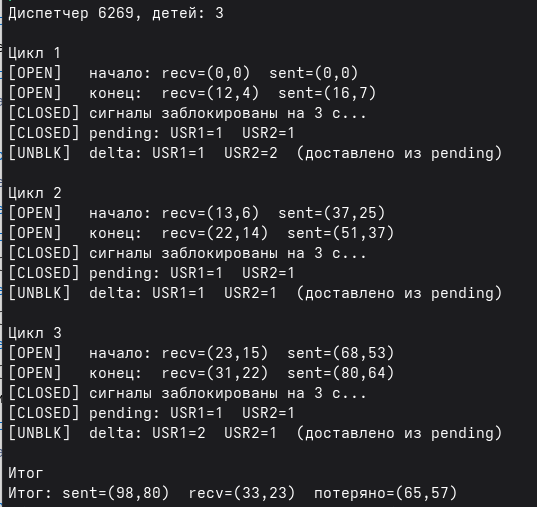
\includegraphics[width = 0.75 \textwidth]{picture/result.png}
        \caption{Результат выполнения программы}
    \end{figure}